\section{3D Deep ResNet Architecture}
\label{sec:model_arch}

\subsection{Design Principles}
\label{sec:design_principles}

Our 3D ResNet variants are designed for volumetric medical imaging with three key principles:
\begin{enumerate}
    \item \textbf{Multi-scale hierarchy:} Three downsampling stages capture features at local (40$^3$), regional (20$^3$), and global (10$^3$) scales, matching striatal anatomy (edges $\to$ sub-regions $\to$ whole-structure asymmetry).
    \item \textbf{Residual learning:} Skip connections enable gradient flow in deeper networks and mitigate vanishing gradients on 4GB VRAM.
    \item \textbf{Channel scaling:} Progressive doubling (16$\to$32$\to$64$\to$128 or 20$\to$40$\to$80$\to$160) balances representational capacity and memory.
\end{enumerate}

\subsection{Net3dR-v25 (Regular)}
\label{sec:net3dr}

\begin{align*}
\text{Input:} &\quad (1, 80, 80, 80) \\
\text{Stem:} &\quad \text{Conv3D}(1\!\to\!16, 3^3, p=1) + \text{BN} + \text{ReLU} + \text{MaxPool3D}(2) \to (16, 40, 40, 40) \\
\text{Stage 1:} &\quad \mathcal{R}(16) \to \mathcal{D}(16\!\to\!32) \to (32, 20, 20, 20) \\
\text{Stage 2:} &\quad \mathcal{D}(32\!\to\!64) \to (64, 10, 10, 10) \\
\text{Stage 3:} &\quad \text{Conv3D}(64\!\to\!128, 3^3, p=1) + \text{BN} + \text{ReLU} \to (128, 10, 10, 10) \\
\text{Head:} &\quad \text{AvgPool3D}(2^3) \to \text{FC}(1024\!\to\!256) \to \text{FC}(256\!\to\!1)
\end{align*}

\textbf{Total parameters: 845,089.}

\subsection{Net3dBig-v25 (Wide)}
\label{sec:net3dbig}

\begin{align*}
\text{Stem:} &\quad \text{Conv3D}(1\!\to\!20, 3^3, p=1) + \text{BN} + \text{ReLU} + \text{MaxPool3D}(2) \to (20, 40, 40, 40) \\
\text{Stage 1:} &\quad \mathcal{R}(20) \to \mathcal{D}(20\!\to\!40) \to (40, 20, 20, 20) \\
\text{Stage 2:} &\quad \mathcal{D}(40\!\to\!80) \to (80, 10, 10, 10) \\
\text{Stage 3:} &\quad \text{Conv3D}(80\!\to\!160, 3^3, p=1) + \text{BN} + \text{ReLU} \to (160, 10, 10, 10) \\
\text{Head:} &\quad \text{AvgPool3D}(2^3) \to \text{FC}(1280\!\to\!320) \to \text{FC}(320\!\to\!1)
\end{align*}

\textbf{Total parameters: 1,319,721.}

\subsection{Residual and Downsampling Blocks}
\label{sec:blocks}

\begin{align*}
\mathcal{R}(x) &= \text{ReLU}\big(x + \text{BN}(\text{Conv}_{3^3}(\text{ReLU}(\text{BN}(\text{Conv}_{3^3}(x)))))\big) \\
\mathcal{D}(x) &= \mathcal{R}\big(\text{BN}(\text{Conv}_{3^3,\text{stride}=2}(x))\big)
\end{align*}

Both convolutions use $3\times3\times3$ kernels with padding=1. Downsampling blocks halve spatial resolution while doubling channels.

\subsection{Configuration Evolution}
\label{sec:arch_evolution}

\begin{table}[htbp]
\centering
\caption{Model architecture evolution across configurations.}
\label{tab:arch_evolution}
\begin{tabular}{lccc}
\toprule
\textbf{Component} & \textbf{Config A (Hybrid)} & \textbf{Config B (CNN-only)} & \textbf{Config C (Deep Ensemble)} \\
\midrule
Architecture family & Net3dR / Net3dBig & Net3dR / Net3dBig & \textbf{Deep ResNet v25} \\
Residual blocks & 2 & 2 & \textbf{3} \\
Downsampling stages & 2 & 2 & \textbf{3} \\
Max channels & 64 / 48 & 64 / 48 & \textbf{128 / 160} \\
Parameters per model & 280K / 294K & 280K / 294K & \textbf{845K / 1.3M} \\
Models in ensemble & 6 (3+3) & 6 (3+3) & \textbf{10 (5+5)} \\
Seeds per architecture & 3 & 3 & \textbf{5} \\
Input resolution & 32$\times$40$\times$48 & 80$^3$ & 80$^3$ \\
Crop/Full volume & Crop & Full & Full \\
\bottomrule
\end{tabular}
\end{table}

\begin{figure}[htbp]
    \centering
    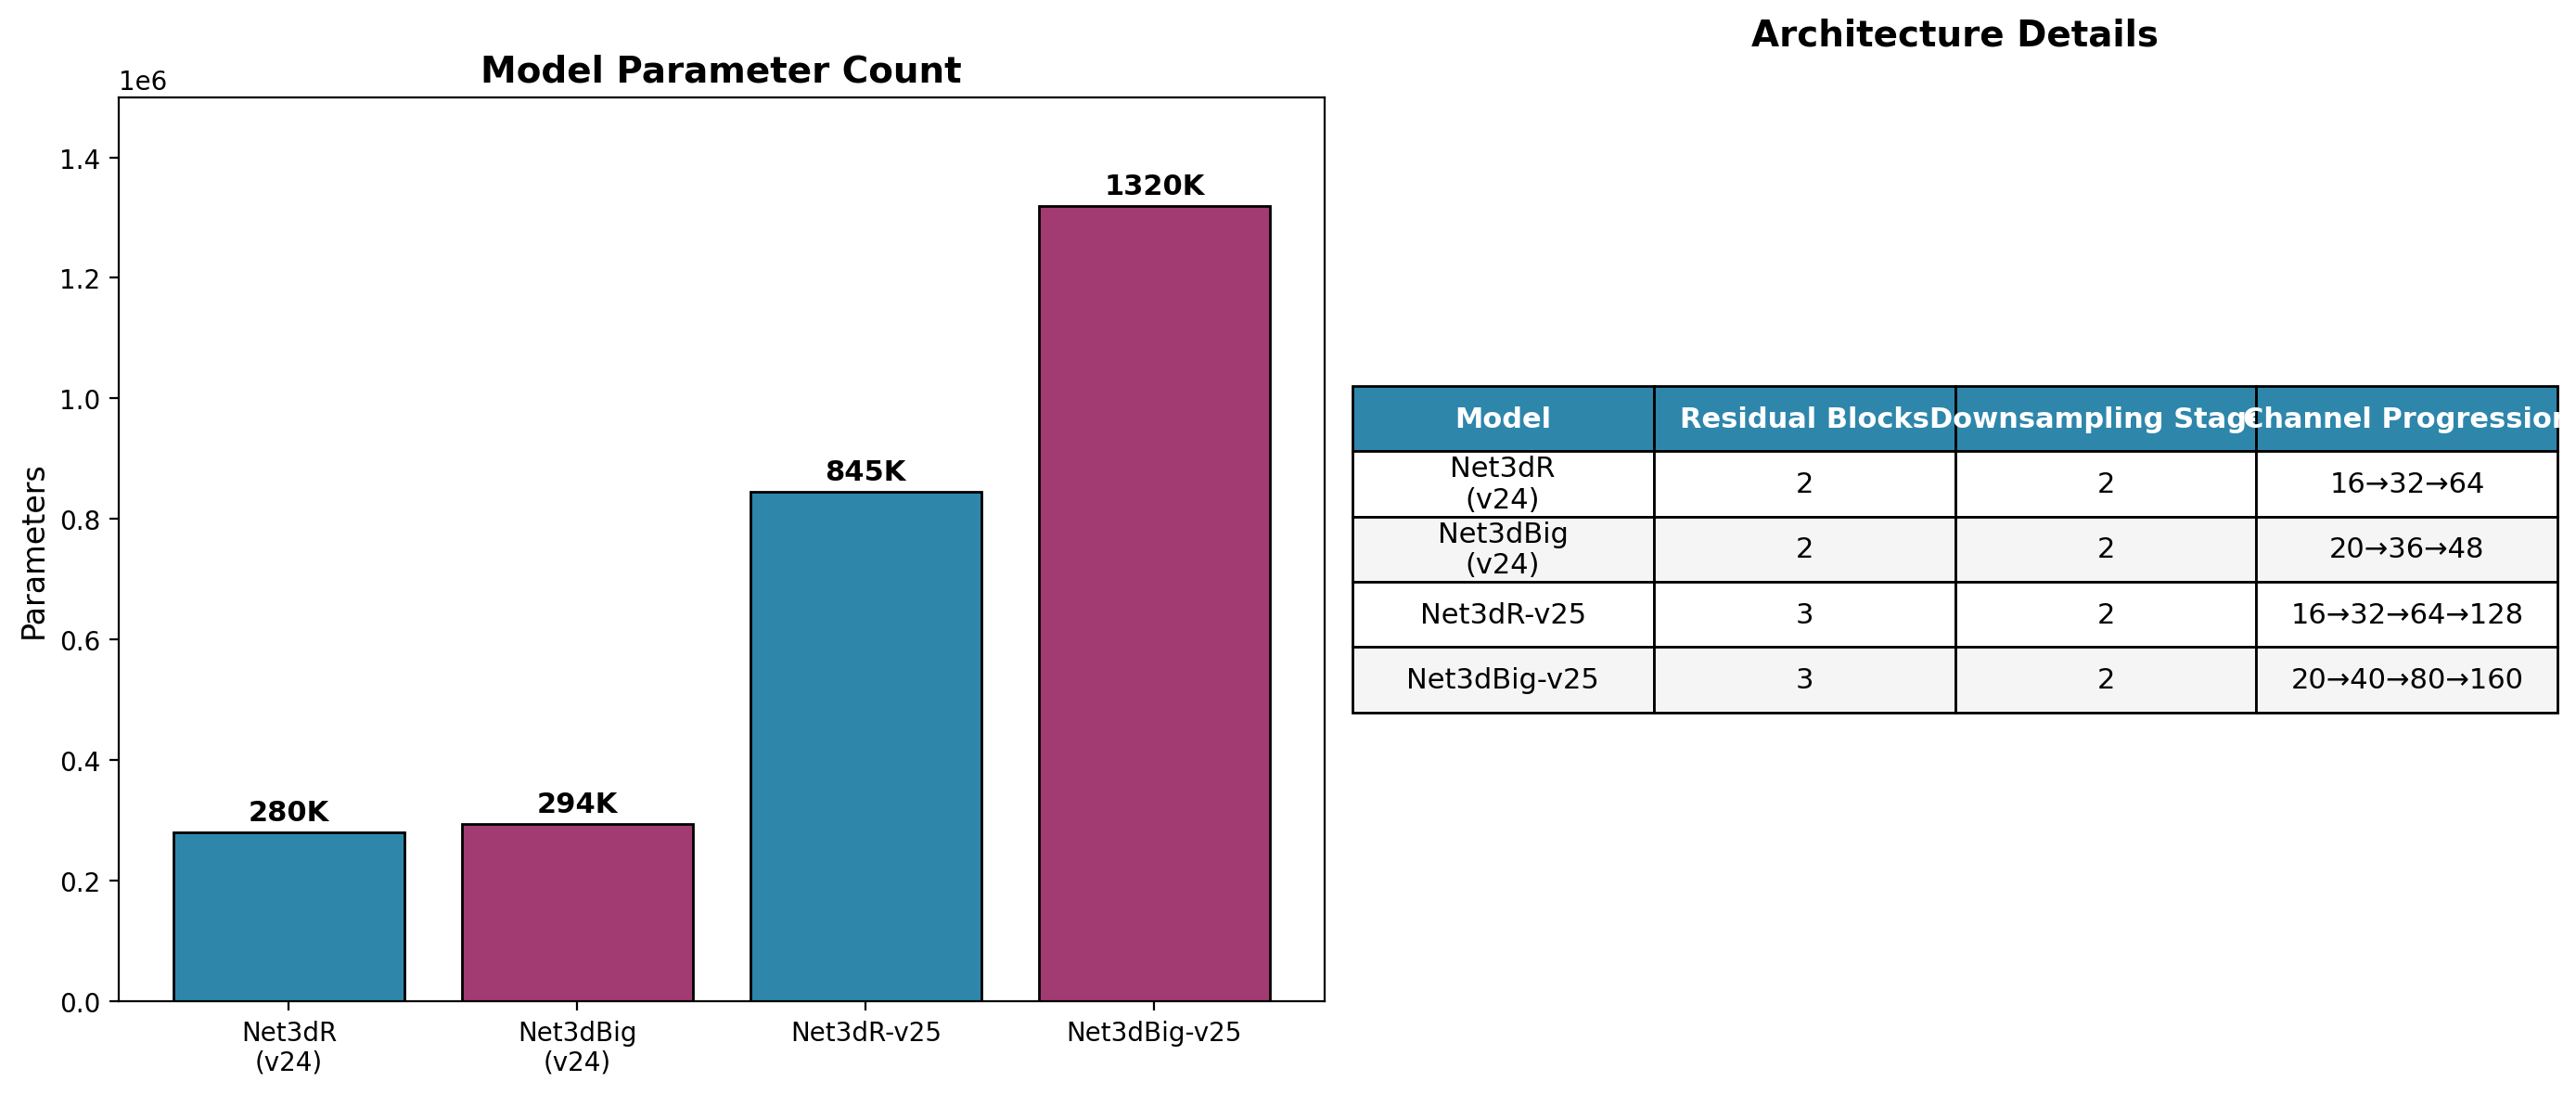
\includegraphics[width=0.95\linewidth]{figures/architecture_comparison.png}
    \caption{Architecture comparison. (Left) Parameter count evolution. (Right) Architecture details table.}
    \label{fig:arch_comparison}
\end{figure}

\subsection{Training Configuration}
\label{sec:training_config}

\begin{table}[htbp]
\centering
\caption{Complete training hyperparameters for Config C models.}
\label{tab:training_hyperparams}
\begin{tabular}{ll}
\toprule
\textbf{Parameter} & \textbf{Value} \\
\midrule
Optimizer & AdamW \\
Learning rate & $10^{-4}$ \\
Weight decay & $10^{-4}$ \\
Batch size (per GPU) & 8 \\
Gradient accumulation & 3 \\
Effective batch size & 24 \\
Max epochs & 100 \\
Early stopping patience & 20 \\
Scheduler & CosineAnnealingLR ($T_{\text{max}}=100$) \\
Mixed precision & AMP (FP16) \\
Gradient clipping & max\_norm=1.0 \\
Seeds per architecture & 5 \\
\midrule
\textbf{Augmentation} & \\
Mixup $\alpha$ & 0.2 \\
Label smoothing $\epsilon$ & 0.05 \\
Random flip prob. & 0.5 (each axis) \\
Random scale range & [0.93, 1.07] \\
Random shift range & [-0.02, 0.02] \\
\bottomrule
\end{tabular}
\end{table}

\textbf{Loss function:} Label-smoothing BCE with Mixup:
\begin{equation}
\mathcal{L} = \mathbb{E}_{(\mathbf{x},y)\sim\mathcal{D}} \Big[ \ell_{\text{BCE}}\big(f(\text{Mix}_\alpha(\mathbf{x})), \text{Mix}_\alpha(y)\big) \Big]
\end{equation}
where $\text{Mix}_\alpha(\mathbf{x}) = \lambda \mathbf{x}_i + (1-\lambda)\mathbf{x}_j$, $\lambda \sim \text{Beta}(\alpha,\alpha)$, $\alpha=0.2$. Label smoothing: $y_{\text{smooth}} = y(1-\epsilon) + 0.5\epsilon$, $\epsilon=0.05$.

\subsection{Ensemble Strategy}
\label{sec:ensemble}

\begin{itemize}
    \item 5 random seeds per architecture: \{42, 777, 2024, 1984, 100\} for Net3dR; \{2025, 314, 271, 1337, 999\} for Net3dBig
    \item Each seed trained independently on all 5 folds (50 models total)
    \item Fold weights averaged for final inference models: $\theta_{\text{final}} = \frac{1}{5}\sum_{f=1}^5 \theta_f$
\end{itemize}

\begin{figure}[htbp]
    \centering
    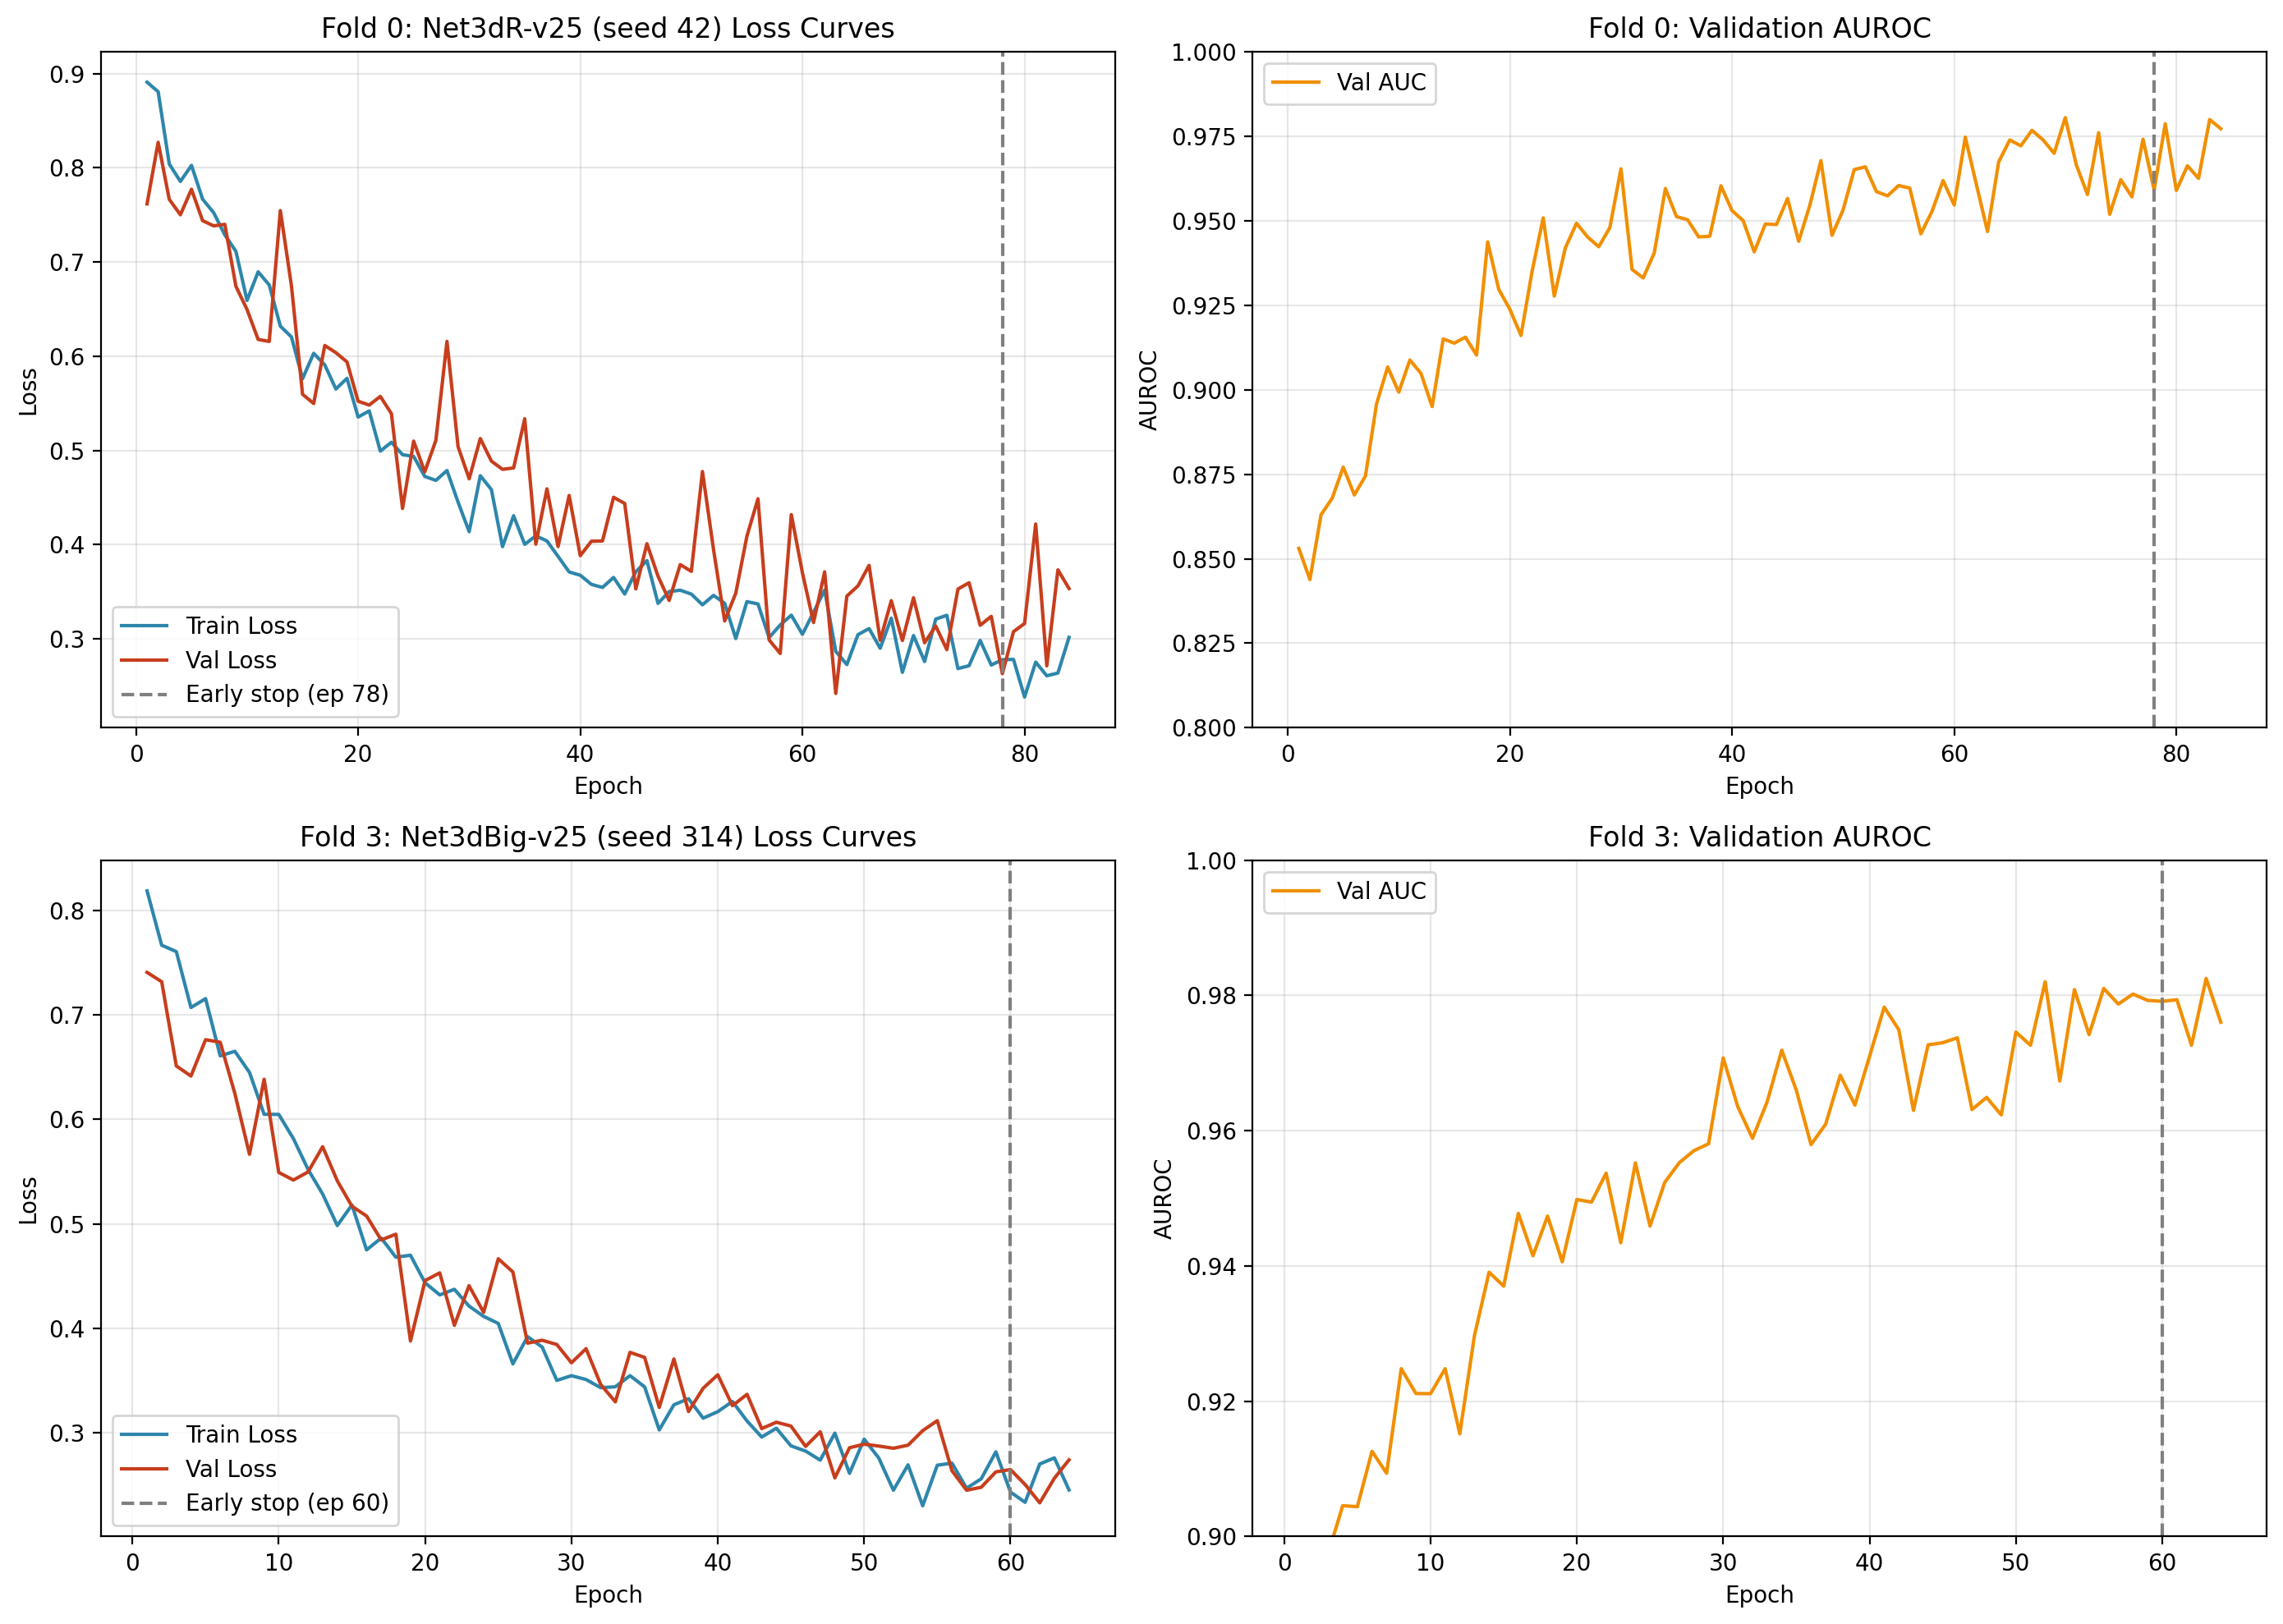
\includegraphics[width=0.95\linewidth]{figures/training_curves.png}
    \caption{Training curves. (Top) Net3dR-Config C Fold 0 seed 42: early stop epoch 78. (Bottom) Net3dBig-Config C Fold 3 seed 314: early stop epoch 60.}
    \label{fig:training_curves}
\end{figure}